
\section{Immagini Multispettrali e Iperspettrali}
Nelle immagini multispettrali, così come in quelle iperspettrali, ogni pixel 
dell’immagine non è costituito da un solo valore monocromatico, 
come nel caso delle immagini pancromatiche (a scala di grigi), o da una terna di valori, 
come nel caso delle immagini a colori RGB, ma da un insieme di valori appartenenti 
allo spettro elettromagnetico. 
Nella scienza del processamento delle immagini, questi valori sono
anche noti come \textbf{Canale} \cite{ALL6_REMOTE_SENSING,immagini_multispettrali2,immagini_multispettrale3,ALL2_REMOTE_SENSING}.

A differenza delle immagini multispettrali, le iperspettrali possiedono un numero elevato di bande, 
che rappresentano intervalli discreti dello spettro elettromagnetico, e producono uno spettro 
continuo per ogni pixel ritratto nella scena. Tipicamente, un'immagine multispettrale
possiede un numero di canali che varia dai 3 fino ad arrivare a 13. In alcuni casi si 
utilizzano anche 15 canali.
Mentre nelle immagini iperspettrali, il numero di canali si aggira intorno alle centinaia:
tipicamente si utilizzano 100 o 200 canali, ma è possibile arrivare anche a numeri ben 
più elevati
\cite{Immagini_multispettrali,immagini_multispettrali2,immagini_multispettrale3,ALL2_REMOTE_SENSING}.
\newpage
La figura (\ref{fig:Multy_vs_Hyper_spectral}) mette in risalto la differenza 
tra queste due tipologie di immagini.

\begin{figure}[H]
    \centering
    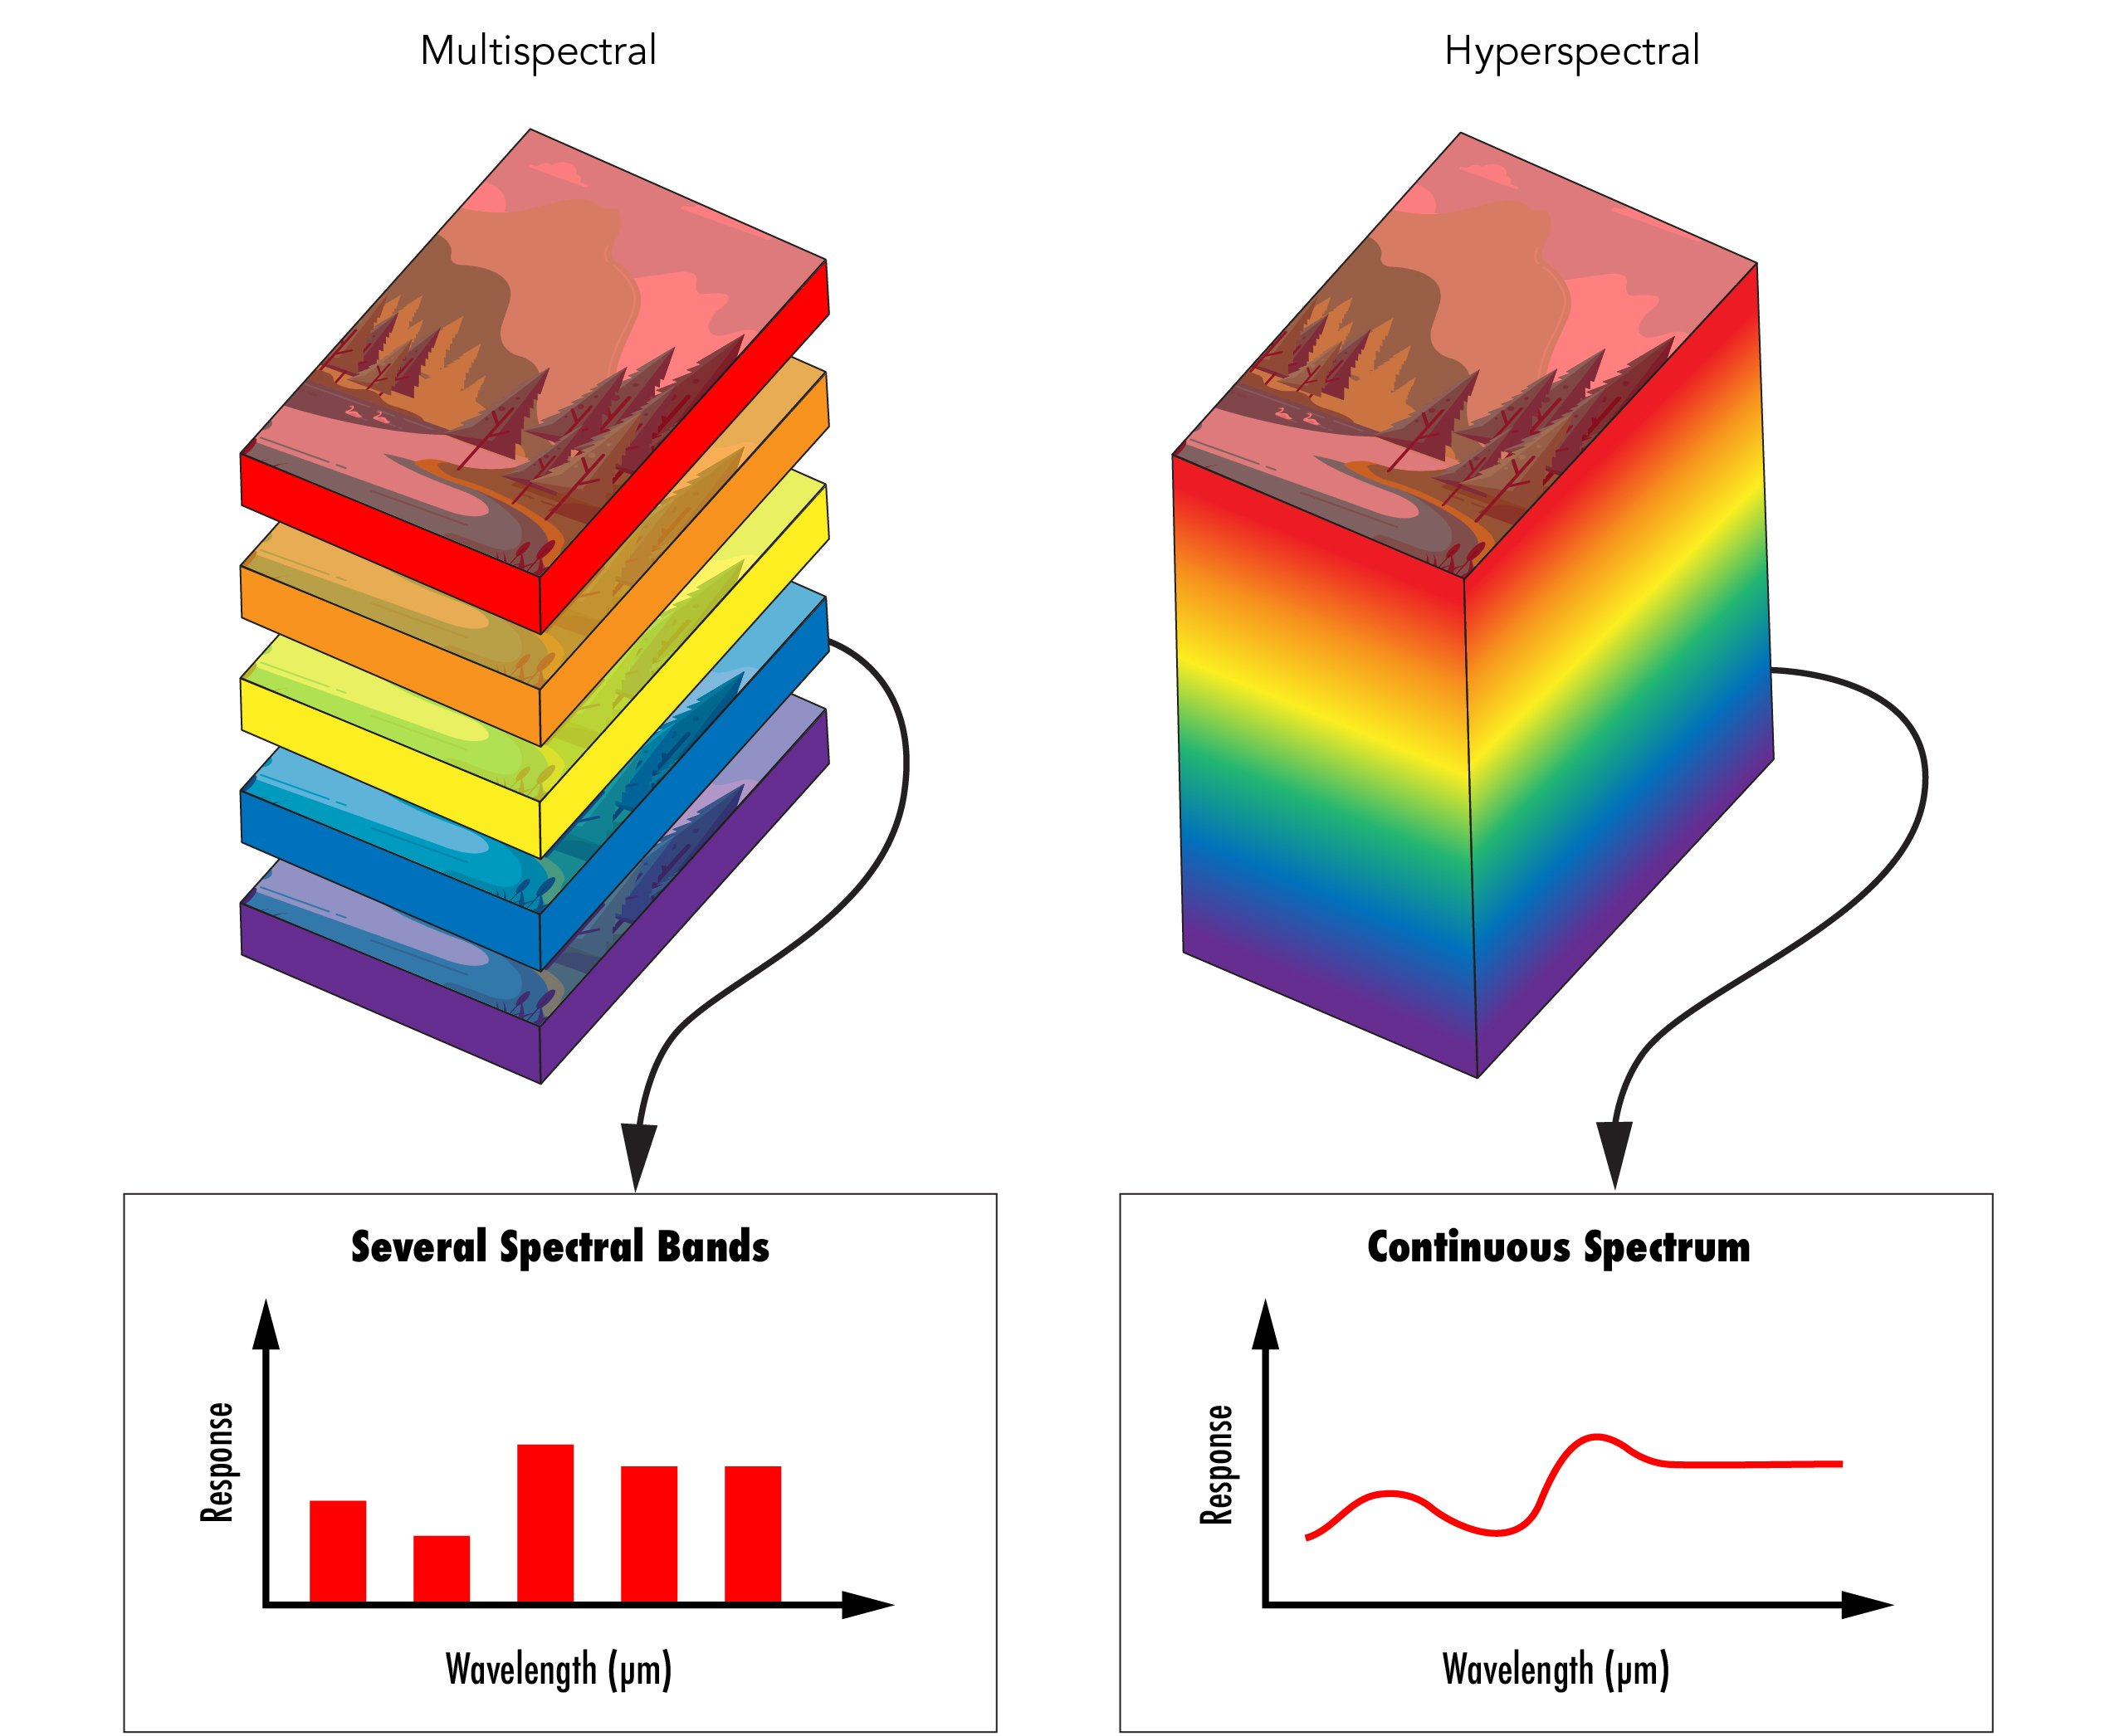
\includegraphics[width=0.60\textwidth]{Immagini/Generiche/Multy_vs_Hyper_spectral.png}
    \caption{ Confronto tra Multispectral e Hyperspectral Imaging \cite{Immagini_multispettrali}.}
    \label{fig:Multy_vs_Hyper_spectral}
    %Figura 2.1: Esempio schematico di un neurone
\end{figure}

Come si può osservare dalla figura \ref{fig:Multy_vs_Hyper_spectral}, 
una singola immagine iperspettrale o multispettrale può essere vista come un 
cubo di dati, in cui le informazioni spaziali sono disposte lungo l'asse X e 
l'asse Y, mentre le informazioni di carattere spettare sono disposte 
lungo l'asse Z \cite{Immagini_multispettrali}.
% Una singola immagine iperspettrale/multispettrale può essere considerata come un 
% cubo di dati, in cui le informazioni spaziali sono raccolte sul piano X-Y, 
% mentre le informazioni spettrali sono rappresentate lungo l’asse Z. 
% Lungo quest’ultima direzione il cubo è costituito da tanti piani quante sono le bande 
% che compongono lo spettro telerilevato.
 

\begin{figure}[H]
    \centering
    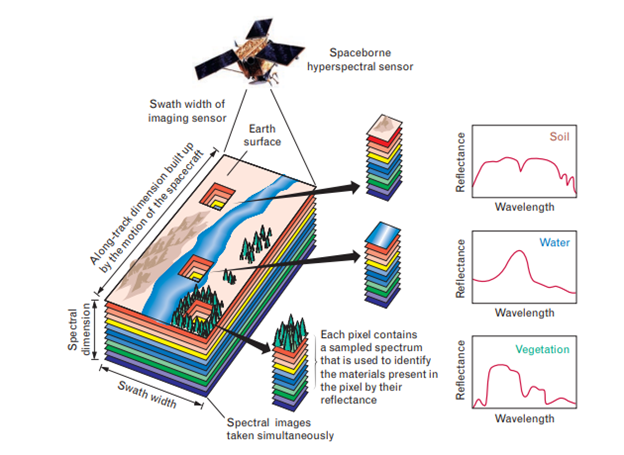
\includegraphics[width=0.80\textwidth]{Immagini/Generiche/scansionamento_terreno.png}
    \caption{Rappresentazione grafica dell'acquisizione di dati \cite{immagini_multispettrali2} .}
    \label{fig:bho1}
    %Figura 2.1: Esempio schematico di un neurone
\end{figure}

% Spesso lo spettro associato ad un pixel è uno spettro di riflettanza, 
% che può contenere fino a centinaia di valori monocromatici. La riflettanza è una 
% grandezza adimensionale, compresa tra 0 e 1, che rappresenta l’efficienza con la 
% quale una superficie riesce a riflettere la luce di una data lunghezza d’onda.

L'utilizzo di diversi canali spettrali fornisce informazioni più complete e accurate 
sulla superficie terrestre. Ogni canale registra informazioni sulla luce in una gamma 
specifica di lunghezze d'onda, che possono essere utili per applicazioni e compiti 
specifici.




 










\subsection{Visualizzazione delle diverse bande}

Le immagini a colori sono composte da 3 canali: il rosso, verde e il blu. Questi canali
vengono sovrapposti per permettere la visualizzazione a colori reali dell'immagine.

\begin{figure}[H]
    \centering
    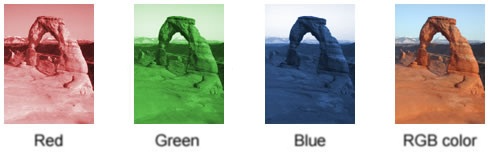
\includegraphics[width=0.60\textwidth]{Immagini/Generiche/canali_rgb.png}
    \caption{Rappresentazione di un immagine a colori.}
    %\label{fig:Classificazion_radiazioni_elettromagnetiche}
\end{figure}

Quando abbiamo un'immagine composta da diverse bande (come le immagini multispettrali e 
iperspettrali), la cosa più semplice (ma in genere meno interessante) che possiamo fare 
è visualizzare singolarmente ogni banda in scala di grigi oppure utilizzare delle heatmap. 

Se vogliamo un'immagine a colori dobbiamo scegliere tre bande a cui assegnare i tre 
colori fondamentali R (Red), G (Green), B (Blue). Se usiamo le bande che corrispondono 
effettivamente a rosso, verde e blu otteniamo un'immagine in colori reali, se invece 
usiamo anche le altre bande avremo un'immagine in falsi colori \cite{immagini_multispettrali_a_colori}.

\begin{figure}[H]
    \centering
    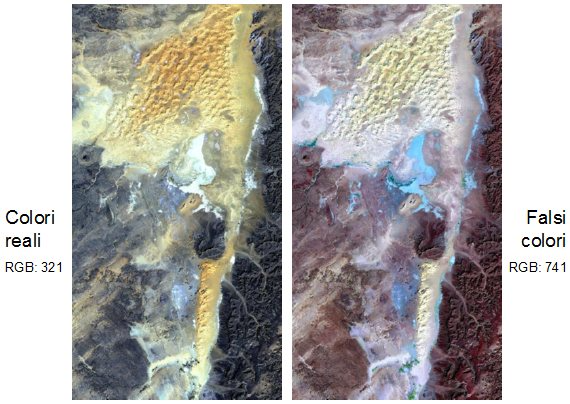
\includegraphics[width=0.75\textwidth]{Immagini/Generiche/paragone_bande.png}
    \caption{Differenze dell'utilizzo di diversi canali \cite{immagini_multispettrali_a_colori} .}
    %\label{fig:Classificazion_radiazioni_elettromagnetiche}
\end{figure}

La combinazione delle diverse bande dipende da cosa vogliamo visualizzare e 
mettere in risalto.